\chapter{La síntesis: rendimiento y pureza}\label{ch:g10:synthesis-yield}

La aspirina es uno de los medicamentos más usados del mundo. Su historia
empieza con la corteza de sauce, que se masticaba desde antiguo contra
el dolor y la fiebre; en el siglo XIX se descubrió que la sustancia
activa de la corteza pertenecía a una familia de compuestos a partir de
los cuales los químicos prepararon el ácido salicílico. Demasiado
agresivo para el estómago para tomarlo en dosis altas, el ácido
salicílico se transformó en una sustancia más suave, el ácido
acetilsalicílico: la aspirina. Hoy se fabrica por toneladas en reactores
de acero, mediante la misma reacción que el laboratorio de un instituto
puede llevar a cabo en una tarde. Fabricar una sustancia es solo la
mitad del trabajo: además hay que separarla de todo lo demás que hay en
el matraz, purificarla, comprobarla y pesarla para ver cuánto se ha
obtenido realmente de lo que era posible.

\begin{recall}
La \omterm{def:g10:chemical-species:extraction}{extracción}, la \omterm{def:g10:chemical-species:distillation}{destilación}, la cromatografía en capa fina y el \omterm{def:g10:chemical-species:retention-factor}{factor
de retención}; un sólido puro funde a una temperatura neta y conocida
(\cref{ch:g10:chemical-species}). Un filtro retiene un sólido y deja
pasar un líquido (\cref{ch:g3:separating-mixtures}). La \omterm{def:g10:reaction-progress-table:extent}{tabla de avance}
da la cantidad máxima de producto a partir del \omterm{def:g10:reaction-progress-table:limiting}{reactivo limitante}
(\cref{ch:g10:reaction-progress-table}).
\end{recall}

\begin{omfigure}
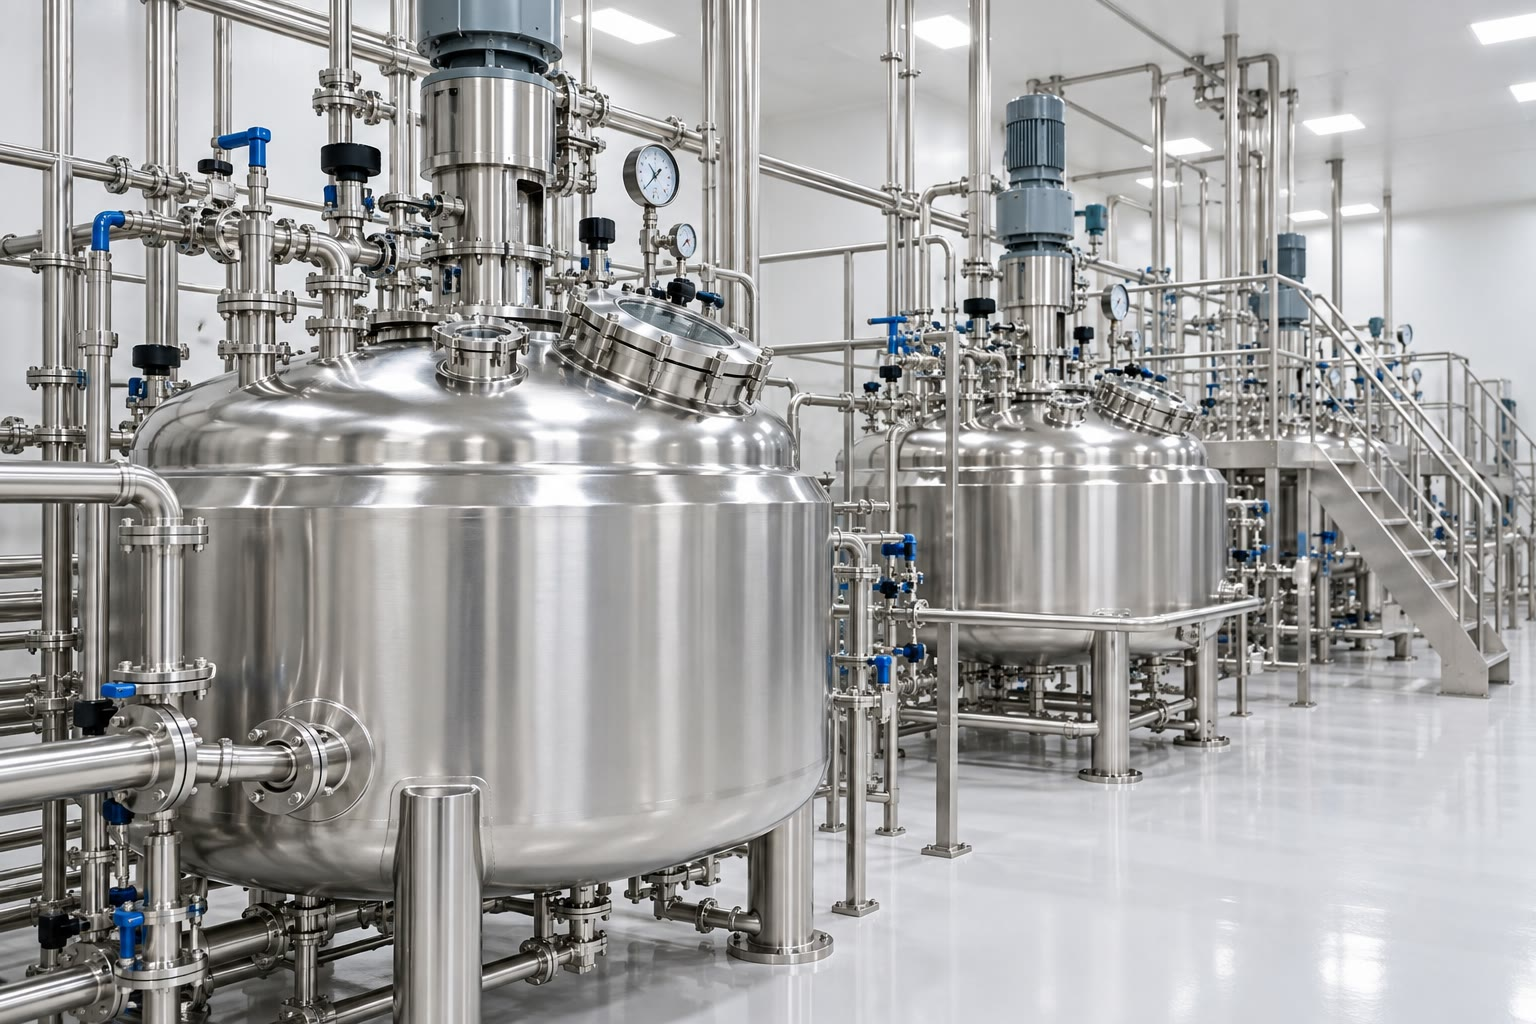
\includegraphics[width=0.55\linewidth]{images/book1/ai/g10-pharma-reactor.jpg}

{\small Reactores de acero de una planta farmacéutica: una \omterm{def:g10:synthesis-yield:synthesis}{síntesis} de
laboratorio, ampliada un millón de veces.}
\end{omfigure}

\section{Las etapas de una síntesis}

\begin{definition}[Síntesis, producto bruto]\label{def:g10:synthesis-yield:synthesis}
Una \emph{síntesis}\index{sintesis@síntesis} es la preparación de una \omterm{def:g6:pure-substances-and-mixtures:species}{especie
química} mediante una o varias \omterm{def:g7:chemical-reactions:reaction}{reacciones químicas}, a partir de otras
especies. El sólido o el líquido que se recupera directamente de la
\omterm{def:g6:pure-substances-and-mixtures:mixture}{mezcla} de reacción, antes de cualquier purificación, es el
\emph{producto bruto}\index{producto bruto}: todavía contiene \omterm{def:g7:chemical-reactions:reactant}{reactivos},
subproductos y \omterm{def:g6:solutions-and-solubility:solute}{disolvente}.
\end{definition}

\begin{method}[Planificar una síntesis]\label{met:g10:synthesis-yield:plan}
Una \omterm{def:g10:synthesis-yield:synthesis}{síntesis} se lleva a cabo en cuatro etapas:
\begin{enumerate}
  \item \textbf{Reacción}: \omterm{def:g2:mixing-and-dissolving:mix}{mezclar} los \omterm{def:g7:chemical-reactions:reactant}{reactivos} en las cantidades
        adecuadas, a menudo con uno en exceso, y calentar si hace falta.
  \item \textbf{Aislamiento}: separar el \omterm{def:g10:synthesis-yield:synthesis}{producto bruto} de la \omterm{def:g6:pure-substances-and-mixtures:mixture}{mezcla} de
        reacción (\omterm{def:g3:separating-mixtures:filter}{filtración}, \omterm{def:g10:chemical-species:extraction}{extracción}).
  \item \textbf{Purificación}: eliminar las impurezas del \omterm{def:g10:synthesis-yield:synthesis}{producto bruto}
        (\omterm{def:g10:synthesis-yield:recrystallisation}{recristalización} para un sólido, \omterm{def:g10:chemical-species:distillation}{destilación} para un líquido).
  \item \textbf{Análisis}: comprobar la identidad y la pureza del
        producto (punto de fusión, cromatografía), y después pesarlo y
        calcular el \omterm{def:g10:synthesis-yield:yield}{rendimiento}.
\end{enumerate}
\end{method}

\begin{example}[Fabricar aspirina]\label{ex:g10:synthesis-yield:aspirin}
El ácido salicílico reacciona con el anhídrido etanoico (llamado también
anhídrido acético) y da aspirina y ácido etanoico:
\[
  \ce{C7H6O3 + C4H6O3 -> C9H8O4 + C2H4O2}
\]
\[
  \text{ácido salicílico} + \text{anhídrido etanoico} \longrightarrow
  \text{aspirina} + \text{ácido etanoico}.
\]
El anhídrido se pone en exceso, para que reaccione todo el ácido
salicílico; el ácido etanoico formado es un subproducto.
\end{example}

\begin{omfigure}
\setchemfig{atom sep=1.7em}
\begin{tabular}{@{}c@{\enspace}c@{\enspace}c@{\enspace}c@{\enspace}c@{\enspace}c@{\enspace}c@{}}
\chemfig{*6(-=-(-COOH)=(-OH)-=)} & $+$ &
\chemfig{H_3C-C(=[2]O)-O-C(=[2]O)-CH_3} & $\longrightarrow$ &
\chemfig{*6(-=-(-COOH)=(-O-[:150]C(=[:90]O)-[:210]H_3C)-=)} & $+$ &
\chemfig{H_3C-C(=[2]O)-OH} \\[2pt]
\small ácido salicílico & & \small anhídrido etanoico & &
\small aspirina & & \small ácido etanoico
\end{tabular}\par\medskip

{\small La fabricación de la aspirina, con fórmulas dibujadas (cada
vértice del hexágono es un \omterm{def:g7:atoms-and-molecules:atom}{átomo} de carbono, que lleva un \omterm{def:g7:atoms-and-molecules:atom}{átomo} de
hidrógeno allí donde no se dibuja nada más; un capítulo posterior
explica esta notación abreviada). El grupo \ce{-OH} del anillo del
ácido salicílico toma la mitad del anhídrido; la otra mitad sale como
ácido etanoico.}
\end{omfigure}

\section{El calentamiento a reflujo}

\begin{definition}[Calentamiento a reflujo]\label{def:g10:synthesis-yield:reflux}
El \emph{calentamiento a reflujo}\index{calentamiento a reflujo}
consiste en calentar una \omterm{def:g6:pure-substances-and-mixtures:mixture}{mezcla} de reacción en un matraz coronado por un
refrigerante vertical: los vapores suben, se enfrían en el refrigerante
y el líquido vuelve a caer al matraz.
\end{definition}

\begin{proposition}[Por qué a reflujo]\label{prop:g10:synthesis-yield:why-reflux}
Calentar acelera la mayoría de las reacciones; el reflujo permite
calentar todo el tiempo necesario a la temperatura de ebullición de la
\omterm{def:g6:pure-substances-and-mixtures:mixture}{mezcla} sin perder en forma de vapor ningún \omterm{def:g7:chemical-reactions:reactant}{reactivo}, producto ni
\omterm{def:g6:solutions-and-solubility:solute}{disolvente}.
\end{proposition}

\begin{proof}
La temperatura de un líquido que hierve no puede subir por encima de su
punto de ebullición, y todo vapor que escapa del líquido se condensa y
vuelve: nada sale del aparato, que se deja abierto por arriba para que
no se acumule presión.
\end{proof}

\begin{omfigure}
\begin{tikzpicture}[font=\small, scale=1.05]
  \pic[transform shape] at (0,0) {heatingmantle};
  \pic[transform shape] at (0,0) {rbflask={0.42}{orange!25}};
  \foreach \p in {(-0.3,0.25), (0.2,0.18), (0.45,0.4), (-0.5,0.5)}
    \fill[black!45] \p circle (0.05);
  \pic[transform shape] at (0,3.0) {condenser};
  \draw[omDef, thick, <-] (0.8,3.825) -- (1.9,3.825) node[right] {entrada de agua};
  \draw[omDef, thick, ->] (0.8,5.375) -- (1.9,5.375) node[right] {salida de agua};
  \draw[omProp, thick, <-] (-0.18,5.8) -- (-1.4,6.1) node[left] {abierto por arriba};
  \draw[omProp, thick, <-] (-0.45,1.2) -- (-2.0,1.6)
    node[left, align=right] {mezcla de reacción\\ y reguladores de ebullición};
  \draw[omProp, thick, <-] (-1.35,-0.2) -- (-2.0,-0.6)
    node[left] {manta calefactora};
  \draw[omThm, ->, thick] (-0.05,3.4) -- (-0.05,4.3);
  \draw[omDef, ->, thick] (0.05,4.3) -- (0.05,3.4);
  \node[omThm, anchor=east, font=\footnotesize] at (-0.45,4.6) {el vapor sube};
  \node[omDef, anchor=west, font=\footnotesize] at (0.85,4.6) {el líquido vuelve a caer};
\end{tikzpicture}

{\small \omterm{def:g10:synthesis-yield:reflux}{Calentamiento a reflujo}. El agua fría entra en la camisa del
refrigerante por abajo y sale por arriba, de modo que la camisa siempre
está llena.}
\end{omfigure}

\begin{remark}[El agua entra por abajo]\label{rem:g10:synthesis-yield:water}
Si entrara por arriba, el agua bajaría directamente y dejaría la parte
superior de la camisa llena de \omterm{def:g4:air-a-mixture-of-gases:air}{aire}; si entra por abajo, tiene que
llenar toda la camisa antes de poder salir.
\end{remark}

\section{Aislar y purificar}

\begin{definition}[Filtración a vacío]\label{def:g10:synthesis-yield:vacuum-filtration}
La \emph{filtración a vacío}\index{filtracion a vacio@filtración a vacío} es una \omterm{def:g3:separating-mixtures:filter}{filtración}
en la que el líquido se hace pasar por el papel de filtro por succión:
un embudo plano con una placa perforada (un embudo Büchner) se coloca
sobre un matraz Kitasato conectado a una bomba de vacío.
\end{definition}

\begin{omfigure}
\begin{tikzpicture}[font=\small, scale=1.05]
  \pic[transform shape] (ff) at (0,0) {filterflask={0.12}{orange!20}};
  \fill[black!50] (-0.3,2.45) rectangle (0.3,2.8);
  \pic[transform shape] at (0,2.45) {buchner={black!8}};
  \draw[black!60, line width=2pt] (ff-arm) -- (2.6,2.2);
  \draw[omProp, thick, ->] (2.7,2.2) -- (3.4,2.2) node[right,
    align=left, text=black] {hacia la\\ bomba de vacío};
  \draw[omProp, thick, <-] (0.7,3.8) -- (1.9,4.3) node[right, text=black]
    {cristales sobre el papel de filtro};
  \draw[omProp, thick, <-] (-0.4,0.15) -- (-1.8,0.6) node[left, text=black]
    {filtrado};
  \draw[omProp, thick, <-] (-0.3,2.6) -- (-1.8,2.9) node[left, text=black]
    {junta de goma};
\end{tikzpicture}

{\small \omterm{def:g10:synthesis-yield:vacuum-filtration}{Filtración a vacío} con un embudo Büchner: la bomba hace pasar el
líquido deprisa y deja el sólido casi seco.}
\end{omfigure}

\begin{definition}[Recristalización]\label{def:g10:synthesis-yield:recrystallisation}
La \emph{recristalización}\index{recristalizacion@recristalización} purifica un sólido
disolviéndolo en el menor volumen posible de un \omterm{def:g6:solutions-and-solubility:solute}{disolvente} caliente y
dejando enfriar después la disolución: el producto, mucho menos soluble
en frío, cristaliza, mientras que las impurezas, presentes en pequeña
cantidad, siguen disueltas.
\end{definition}

\begin{method}[Recristalizar un sólido]\label{met:g10:synthesis-yield:recrystallise}
\begin{enumerate}
  \item Elegir un \omterm{def:g6:solutions-and-solubility:solute}{disolvente} en el que el producto sea muy soluble en
        caliente y poco soluble en frío.
  \item Añadir el \omterm{def:g6:solutions-and-solubility:solute}{disolvente} caliente poco a poco al sólido bruto, justo
        hasta que se haya disuelto todo.
  \item Dejar enfriar la disolución despacio y luego en un baño de
        hielo: se forman cristales.
  \item Recogerlos por \omterm{def:g10:synthesis-yield:vacuum-filtration}{filtración a vacío}, lavarlos con un poco de
        \omterm{def:g6:solutions-and-solubility:solute}{disolvente} muy frío y secarlos.
\end{enumerate}
\end{method}


\begin{omfigure}
\begin{tikzpicture}[font=\small]
  % 1. crude solid + a little hot solvent, on a hot plate
  \pic at (0,0.3) {hotplate};
  \pic at (0,0.3) {erlenmeyer={0.18}{orange!12}};
  \foreach \p in {(-0.4,0.42),(-0.15,0.38),(0.1,0.45),(0.35,0.4),(-0.3,0.55),(0.2,0.6)}
    \fill[brown!60] \p circle (0.06);
  \node[align=center, anchor=north] at (0,-0.15) {1. sólido bruto,\\ disolvente caliente};
  % 2. clear hot solution
  \pic at (3,0.3) {hotplate};
  \pic at (3,0.3) {erlenmeyer={0.22}{orange!12}};
  \node[align=center, anchor=north] at (3,-0.15) {2. todo disuelto,\\ transparente y caliente};
  % 3. ice bath: crystals
  \fill[cyan!12, draw=black!40] (5.0,0) rectangle (7.0,1.2);
  \foreach \p in {(5.2,0.9),(6.75,1.0),(5.3,0.3),(6.8,0.25)}
    \draw[black!35, fill=white] \p ++(-0.12,-0.1) rectangle ++(0.24,0.2);
  \pic at (6,0.1) {erlenmeyer={0.2}{orange!8}};
  \foreach \x/\y in {-0.45/0.18,-0.25/0.15,0/0.2,0.25/0.15,0.45/0.2,-0.1/0.3,0.15/0.32,
                     -0.35/0.32,0.35/0.33}
    \fill[white, draw=black!55] (6+\x,0.1+\y) -- ++(0.07,0.06) -- ++(0.07,-0.06)
      -- ++(-0.07,-0.06) -- cycle;
  \node[align=center, anchor=north] at (6,-0.15) {3. enfriar en hielo:\\ se forman cristales};
  % 4. filter
  \pic at (9,0) {filterflask={0.12}{orange!12}};
  \pic at (9,2.45) {buchner={black!12}};
  \fill[black!50] (8.7,2.45) rectangle (9.3,2.8);
  \node[align=center, anchor=north] at (9,-0.15) {4. filtrar a vacío,\\ lavar en frío, secar};
\end{tikzpicture}

{\small La \omterm{def:g10:synthesis-yield:recrystallisation}{recristalización} en cuatro pasos. Las impurezas siguen
disueltas en el \omterm{def:g6:solutions-and-solubility:solute}{disolvente} frío y pasan al \omterm{def:g3:separating-mixtures:filter}{filtrado}.}
\end{omfigure}

\begin{remark}[Las pérdidas son inevitables]\label{rem:g10:synthesis-yield:losses}
% ledger: sol:aspirin-25, sol:aspirin-37
Incluso en frío, el \omterm{def:g6:solutions-and-solubility:solute}{disolvente} mantiene disuelto algo de producto. La
aspirina se \omterm{def:g2:mixing-and-dissolving:dissolve}{disuelve} en agua a razón de unos \qty{3.3}{g/L} a
\qty{25}{\celsius}, el triple a \qty{37}{\celsius} y mucho más en
caliente: cada mililitro de \omterm{def:g3:separating-mixtures:filter}{filtrado} y de agua de lavado se lleva un
poco de aspirina. Una \omterm{def:g10:synthesis-yield:recrystallisation}{recristalización} compra pureza al precio de masa.
\end{remark}

\section{Analizar el producto}

\begin{proposition}[Dos comprobaciones de pureza]\label{prop:g10:synthesis-yield:checks}
Un sólido sintetizado es puro, dentro de los límites de estas pruebas,
cuando:
\begin{itemize}
  \item funde de forma neta al punto de fusión que dan las tablas;
  \item en una placa de cromatografía en capa fina, da una sola mancha,
        a la misma altura que una muestra de la \omterm{def:g6:pure-substances-and-mixtures:pure-substance}{sustancia pura}.
\end{itemize}
\end{proposition}

\begin{proof}
Se admite: una impureza baja el punto de fusión y lo extiende en un
intervalo (\cref{ch:g10:chemical-species}), y una segunda especie
recorre por lo general una distancia distinta sobre la placa.
\end{proof}

\begin{omfigure}
\begin{tikzpicture}[font=\small, scale=1.3]
  \pic[transform shape] at (0,0) {tlcplate};
  \draw[black!50, dashed] (-0.7,2.7) -- (0.7,2.7);
  % lanes: C crude, R recrystallised, A aspirin, S salicylic acid
  \foreach \x/\l in {-0.5/C,-0.17/R,0.17/A,0.5/S}
    \node[font=\footnotesize, anchor=north] at (\x,0.38) {\l};
  \fill[omDef!70] (-0.5,1.75) ellipse (0.09 and 0.06);
  \fill[omDef!40] (-0.5,1.25) ellipse (0.09 and 0.06);
  \fill[omDef!70] (-0.17,1.75) ellipse (0.09 and 0.06);
  \fill[omDef!70] (0.17,1.75) ellipse (0.09 and 0.06);
  \fill[omDef!70] (0.5,1.25) ellipse (0.09 and 0.06);
  \node[anchor=west, font=\footnotesize] at (0.85,2.7) {frente del eluyente};
  \node[anchor=west, font=\footnotesize] at (0.85,0.4) {línea de partida};
\end{tikzpicture}

{\small Cromatografía del \omterm{def:g10:synthesis-yield:synthesis}{producto bruto} (C) y del producto
recristalizado (R) junto a aspirina pura (A) y ácido salicílico (S),
vista con luz ultravioleta. El \omterm{def:g10:synthesis-yield:synthesis}{producto bruto} todavía contiene ácido
salicílico; el recristalizado, no.}
\end{omfigure}

\section{El rendimiento}

\begin{definition}[Rendimiento]\label{def:g10:synthesis-yield:yield}
El \emph{rendimiento}\index{rendimiento} $\eta$ de una \omterm{def:g10:synthesis-yield:synthesis}{síntesis} es el
cociente entre la cantidad de producto obtenida realmente, pura y seca,
y la cantidad máxima que podría dar el \omterm{def:g10:reaction-progress-table:limiting}{reactivo limitante}:
\[
  \eta = \frac{n_{\text{obtenida}}}{n_{\max}} ,
\]
que se suele dar en tanto por ciento.
\end{definition}

\begin{proposition}[El rendimiento a partir de las masas]\label{prop:g10:synthesis-yield:masses}
Como la cantidad obtenida y la cantidad máxima se refieren al mismo
producto, de \omterm{def:g10:the-mole:molar-mass}{masa molar} $M$, el \omterm{def:g10:synthesis-yield:yield}{rendimiento} es también el cociente de
las masas:
\[
  \eta = \frac{m_{\text{obtenida}}}{m_{\max}},
  \qquad m_{\max} = n_{\max} \times M,
\]
donde $n_{\max}$ sale de la \omterm{def:g10:reaction-progress-table:extent}{tabla de avance}, en $x = x_{\max}$.
\end{proposition}

\begin{proof}
$m_{\text{obtenida}} / m_{\max} = (n_{\text{obtenida}} M) / (n_{\max} M)
= n_{\text{obtenida}} / n_{\max}$.
\end{proof}

\begin{example}[Rendimiento de una síntesis pequeña]\label{ex:g10:synthesis-yield:small}
% ledger: aw:C, aw:H, aw:O
\qty{1.38}{g} de ácido salicílico ($M = \qty{138.0}{g/mol}$), es decir,
\qty{0.0100}{mol}, reaccionan con anhídrido etanoico en exceso. La
cantidad máxima de aspirina es \qty{0.0100}{mol}, es decir,
$0.0100 \times 180.0 = \qty{1.80}{g}$. Si se obtienen \qty{1.35}{g} de
aspirina pura y seca, $\eta = 1.35 / 1.80 = 0.75$, un \omterm{def:g10:synthesis-yield:yield}{rendimiento} del
\qty{75}{\percent}.
\end{example}

\begin{remark}[Por qué los rendimientos son inferiores al 100 \%]\label{rem:g10:synthesis-yield:below}
En cada etapa se pierde producto: pegado al material de vidrio, disuelto
en el \omterm{def:g3:separating-mixtures:filter}{filtrado} y en las aguas de lavado, abandonado en una
\omterm{def:g10:synthesis-yield:recrystallisation}{recristalización}; algunas reacciones dan además productos secundarios,
o se detienen antes de que se agote el \omterm{def:g10:reaction-progress-table:limiting}{reactivo limitante}. Un
\omterm{def:g10:synthesis-yield:yield}{rendimiento} superior al \qty{100}{\percent} indica siempre un error, casi
siempre un producto pesado todavía húmedo o impuro.
\end{remark}

\begin{inthelab}[Fabricar aspirina]
En un matraz seco, el profesor \omterm{def:g6:pure-substances-and-mixtures:mixture}{mezcla} ácido salicílico con un exceso de
anhídrido etanoico y unas gotas de un ácido que acelera la reacción, y
calienta la \omterm{def:g6:pure-substances-and-mixtures:mixture}{mezcla} a reflujo en un baño de agua a unos
\qty{80}{\celsius} durante un cuarto de hora. Tras enfriar, se añade
agua fría: el anhídrido en exceso reacciona con ella, y la aspirina, muy
poco soluble en agua fría, aparece en forma de cristales blancos. Estos
se recogen por \omterm{def:g10:synthesis-yield:vacuum-filtration}{filtración a vacío}, se recristalizan, se secan, se pesan
y se mide su punto de fusión.
\end{inthelab}

\begin{safety}{\ghs[0.82cm]{GHS02}\ghs[0.82cm]{GHS05}\ghs[0.82cm]{GHS06}\ghs[0.82cm]{GHS07}}
% ledger: ghs:acetic-anhydride, ghs:salicylic, ghs:aspirin
El anhídrido etanoico es inflamable, nocivo en caso de ingestión o de inhalación, y provoca
quemaduras graves en la piel y en los ojos: lo manipula el profesor,
bajo una campana extractora, con guantes y gafas. El ácido salicílico es
nocivo en caso de ingestión y puede dañar los ojos. La aspirina hecha en
un laboratorio no se toma nunca como medicamento.
\end{safety}

\begin{omfigure}
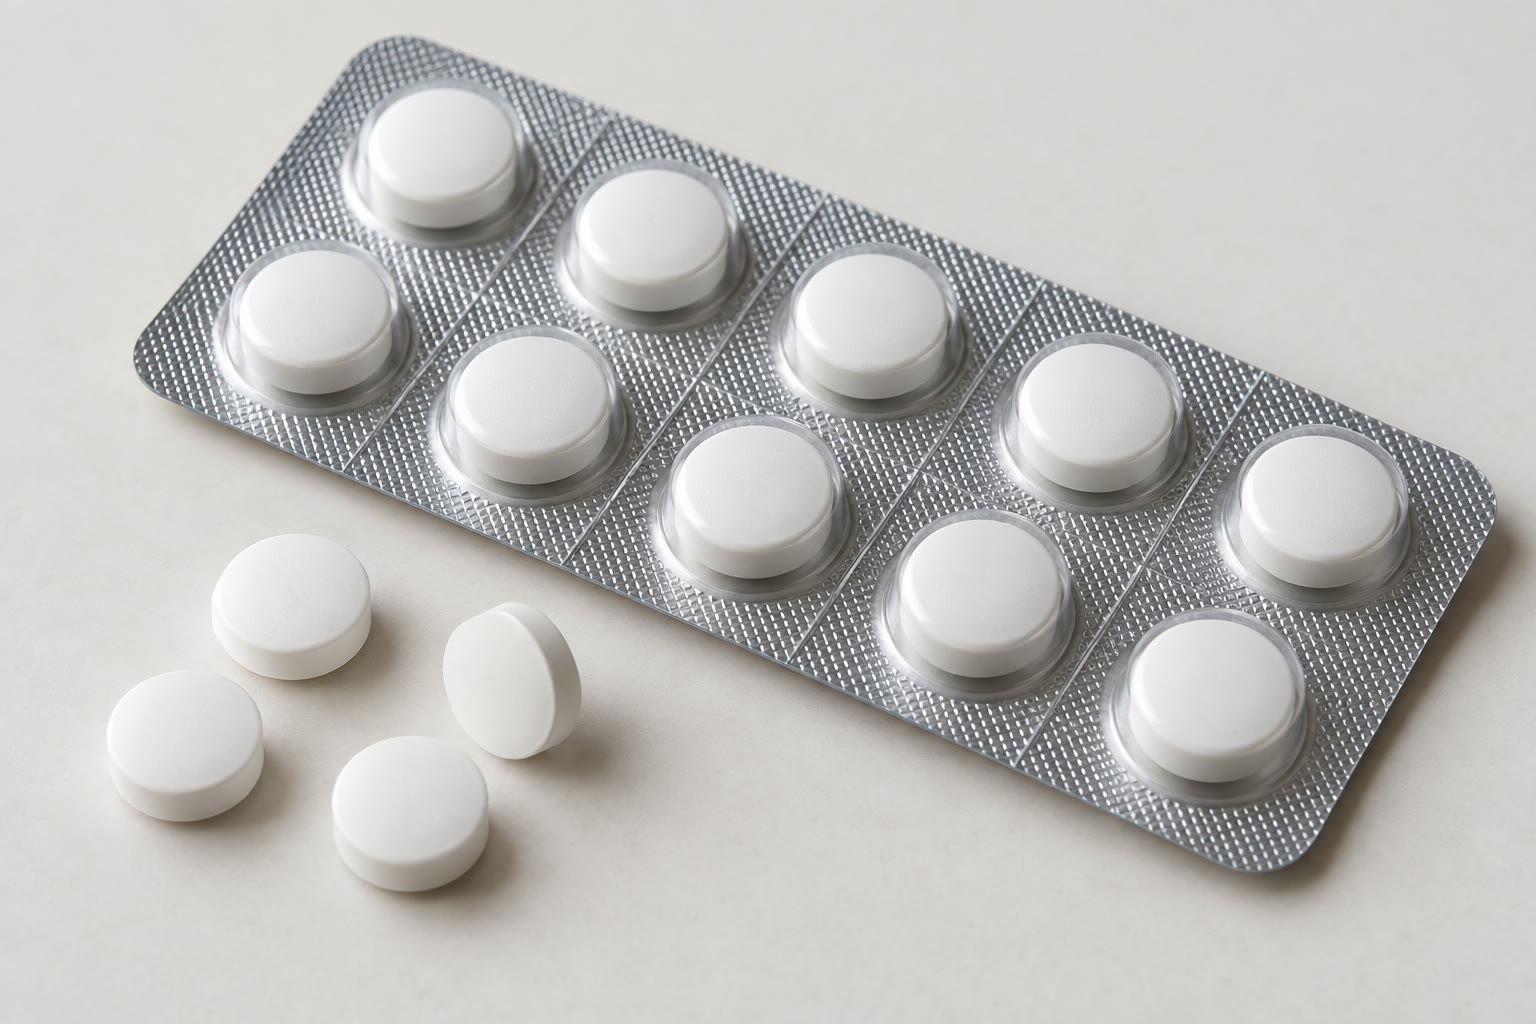
\includegraphics[width=0.45\linewidth]{images/book1/ai/g10-aspirin-tablets.jpg}

{\small Comprimidos de aspirina: cada uno contiene una masa pesada de la
\omterm{def:g6:pure-substances-and-mixtures:pure-substance}{sustancia pura}, \omterm{def:g2:mixing-and-dissolving:mix}{mezclada} con un aglutinante.}
\end{omfigure}

\section{Ejercicios}


\begin{exercise}[$\star$]\label{exo:g10:synthesis-yield:1}
Una \omterm{def:g10:synthesis-yield:synthesis}{síntesis} podría dar como mucho \qty{5.0}{g} de producto; se obtienen
\qty{4.2}{g} de producto puro y seco. Calcula el \omterm{def:g10:synthesis-yield:yield}{rendimiento}.
\end{exercise}

\begin{exercise}[$\star$]\label{exo:g10:synthesis-yield:2}
Ordena estas etapas de una \omterm{def:g10:synthesis-yield:synthesis}{síntesis}: medir el punto de fusión; calentar
a reflujo; recristalizar; filtrar a vacío el \omterm{def:g10:synthesis-yield:synthesis}{producto bruto}; pesar los
\omterm{def:g7:chemical-reactions:reactant}{reactivos}.
\end{exercise}

\begin{exercise}[$\star$]\label{exo:g10:synthesis-yield:3}
En un montaje a reflujo, ¿por qué el agua de refrigeración entra en el
refrigerante por abajo? ¿Por qué se deja abierta la parte superior del
refrigerante?
\end{exercise}

\begin{exercise}[$\star$]\label{exo:g10:synthesis-yield:4}
¿Qué dos propiedades debe tener un \omterm{def:g6:solutions-and-solubility:solute}{disolvente} para recristalizar un
producto? ¿Dónde acaban las impurezas?
\end{exercise}

\begin{exercise}[$\star$]\label{exo:g10:synthesis-yield:5}
% ledger: mp:aspirin
Una muestra de aspirina sintetizada funde entre \qty{124}{\celsius} y
\qty{130}{\celsius}. La aspirina pura funde a unos \qty{135}{\celsius}.
¿Es pura la muestra? ¿Qué habría que hacer?
\end{exercise}

\begin{exercise}[$\star\star$]\label{exo:g10:synthesis-yield:6}
\qty{2.00}{g} de ácido salicílico reaccionan con anhídrido etanoico en
exceso; se obtienen \qty{2.03}{g} de aspirina pura y seca. Calcula la
masa máxima de aspirina y el \omterm{def:g10:synthesis-yield:yield}{rendimiento}.
\end{exercise}

\begin{exercise}[$\star\star$]\label{exo:g10:synthesis-yield:7}
Una alumna pesa su aspirina cuando todavía está húmeda y obtiene un
\omterm{def:g10:synthesis-yield:yield}{rendimiento} del \qty{104}{\percent}. Explícalo. Pesar el \omterm{def:g10:synthesis-yield:synthesis}{producto bruto},
sin purificar pero seco, ¿daría un \omterm{def:g10:synthesis-yield:yield}{rendimiento} demasiado alto o
demasiado bajo con respecto al \omterm{def:g10:synthesis-yield:yield}{rendimiento} real?
\end{exercise}

\begin{exercise}[$\star\star$]\label{exo:g10:synthesis-yield:8}
Da dos ventajas de la \omterm{def:g10:synthesis-yield:vacuum-filtration}{filtración a vacío} frente a una \omterm{def:g3:separating-mixtures:filter}{filtración}
ordinaria con un cono de papel, para recoger cristales.
\end{exercise}

\begin{exercise}[$\star\star$]\label{exo:g10:synthesis-yield:9}
En una placa de cromatografía, el frente del \omterm{def:g10:chemical-species:tlc}{eluyente} ha recorrido
\qty{5.0}{cm}. La mancha de un producto sintetizado ha recorrido
\qty{3.1}{cm}; la de aspirina pura, \qty{3.1}{cm}; la de ácido
salicílico, \qty{2.2}{cm}. Calcula los tres \omterm{def:g10:chemical-species:retention-factor}{factores de retención}. ¿Qué
se puede concluir sobre el producto?
\end{exercise}

\begin{exercise}[$\star\star$]\label{exo:g10:synthesis-yield:10}
La \omterm{def:g6:solutions-and-solubility:solubility}{solubilidad} de un producto en dos \omterm{def:g6:solutions-and-solubility:solute}{disolventes} es:
\begin{center}
\begin{tabular}{lcc}
\hline
\omterm{def:g6:solutions-and-solubility:solute}{disolvente} & en frío (\qty{20}{\celsius}) & en caliente (cerca de la ebullición) \\
\hline
A & \qty{2}{g/L} & \qty{150}{g/L} \\
B & \qty{80}{g/L} & \qty{120}{g/L} \\
\hline
\end{tabular}
\end{center}
¿Qué \omterm{def:g6:solutions-and-solubility:solute}{disolvente} es mejor para una \omterm{def:g10:synthesis-yield:recrystallisation}{recristalización}? Para \qty{3.0}{g}
de \omterm{def:g10:synthesis-yield:synthesis}{producto bruto}, ¿qué volumen de \omterm{def:g6:solutions-and-solubility:solute}{disolvente} caliente hace falta, más o
menos, y qué masa, como mucho, sigue disuelta una vez en frío?
\end{exercise}

\begin{exercise}[$\star\star$]\label{exo:g10:synthesis-yield:11}
¿Por qué el matraz de fondo redondo de un montaje a reflujo nunca está
lleno más que hasta la mitad? ¿Por qué se añaden reguladores de
ebullición?
\end{exercise}

\begin{exercise}[$\star\star\star$]\label{exo:g10:synthesis-yield:12}
Un medicamento se fabrica en dos etapas, de \omterm{def:g10:synthesis-yield:yield}{rendimientos}
\qty{80}{\percent} y \qty{70}{\percent}. ¿Cuál es el \omterm{def:g10:synthesis-yield:yield}{rendimiento} global?
¿Cuál sería para tres etapas del \qty{90}{\percent} cada una? ¿Por qué
los químicos intentan fabricar los medicamentos en el menor número
posible de etapas?
\end{exercise}

\begin{exercise}[$\star\star\star$]\label{exo:g10:synthesis-yield:13}
% ledger: sol:aspirin-25
La aspirina se \omterm{def:g2:mixing-and-dissolving:dissolve}{disuelve} en agua a razón de unos \qty{3.3}{g/L} a
\qty{25}{\celsius}. Se lavan unos cristales con \qty{50}{mL} de agua a
esa temperatura. ¿Qué masa de aspirina se puede perder como mucho? ¿Por
qué se enfría antes el agua de lavado en hielo?
\end{exercise}

\begin{exercise}[$\star\star\star$]\label{exo:g10:synthesis-yield:14}
Se \omterm{def:g2:mixing-and-dissolving:mix}{mezclan} \qty{2.76}{g} de ácido salicílico con \qty{0.0500}{mol} de
anhídrido etanoico. Después de la reacción se añade agua, que destruye
el anhídrido en exceso: \ce{C4H6O3 + H2O -> 2C2H4O2}.
\begin{enumerate}
  \item Rellena la \omterm{def:g10:reaction-progress-table:extent}{tabla de avance} de la \omterm{def:g10:synthesis-yield:synthesis}{síntesis}; ¿qué cantidad de
        anhídrido queda?
  \item ¿Qué cantidad total de ácido etanoico hay al final?
\end{enumerate}
\end{exercise}

\begin{exercise}[$\star\star\star$]\label{exo:g10:synthesis-yield:15}
Una fábrica tiene que producir \qty{1.00}{t} de aspirina, con un
\omterm{def:g10:synthesis-yield:yield}{rendimiento} global del \qty{85}{\percent} a partir del ácido salicílico.
¿Qué masa de ácido salicílico tiene que comprar?
\end{exercise}

\section{Problema: Fabricar aspirina}

\begin{problem}[{Problema de fin de semana --- de tres gramos de ácido
salicílico a un frasco de aspirina pura: ¿cuál es el rendimiento?}]
\label{pb:g10:synthesis-yield:1}
% ledger: rho:acetic-anhydride, mp:aspirin, mp:salicylic, sol:aspirin-25, aw:C, aw:H, aw:O
Una clase fabrica aspirina. En el matraz: \qty{3.0}{g} de ácido
salicílico y \qty{6.0}{mL} de anhídrido etanoico, de densidad
\qty{1.08}{g/mL}, con unas gotas de ácido; la \omterm{def:g6:pure-substances-and-mixtures:mixture}{mezcla} se calienta a
reflujo. El \omterm{def:g10:synthesis-yield:synthesis}{producto bruto} recogido por \omterm{def:g10:synthesis-yield:vacuum-filtration}{filtración a vacío} pesa
\qty{3.6}{g} húmedo y \qty{3.3}{g} una vez seco. Después de la
\omterm{def:g10:synthesis-yield:recrystallisation}{recristalización} y el secado quedan \qty{2.7}{g} de cristales blancos.

\medskip
\noindent\textbf{Parte I --- La reacción.}
\begin{enumerate}
  \item Comprueba que la ecuación
        \ce{C7H6O3 + C4H6O3 -> C9H8O4 + C2H4O2} está ajustada.
  \item Calcula las \omterm{def:g10:the-mole:molar-mass}{masas molares} del ácido salicílico, el anhídrido
        etanoico, la aspirina y el ácido etanoico.
  \item Nombra los \omterm{def:g7:chemical-reactions:reactant}{reactivos}, el producto buscado y el subproducto.
  \item ¿Por qué se calienta la \omterm{def:g6:pure-substances-and-mixtures:mixture}{mezcla} a reflujo y no en un matraz
        abierto?
\end{enumerate}

\medskip
\noindent\textbf{Parte II --- La masa máxima.}
\begin{enumerate}[resume]
  \item Calcula la cantidad inicial de ácido salicílico.
  \item Calcula la masa y después la cantidad de anhídrido etanoico.
  \item Rellena la \omterm{def:g10:reaction-progress-table:extent}{tabla de avance}. ¿Qué \omterm{def:g7:chemical-reactions:reactant}{reactivo} es el limitante? Da
        $x_{\max}$.
  \item Deduce la masa máxima de aspirina.
  \item ¿Por qué se pone en exceso el anhídrido, y no el ácido
        salicílico?
\end{enumerate}

\medskip
\noindent\textbf{Parte III --- Aislar y purificar.}
\begin{enumerate}[resume]
  \item ¿Por qué no se puede usar la masa húmeda, \qty{3.6}{g}, para
        calcular un \omterm{def:g10:synthesis-yield:yield}{rendimiento}?
  \item Calcula el \omterm{def:g10:synthesis-yield:yield}{rendimiento} en \omterm{def:g10:synthesis-yield:synthesis}{producto bruto} seco.
  \item ¿Por qué la \omterm{def:g10:synthesis-yield:recrystallisation}{recristalización} hace bajar la masa?
  \item Los cristales se lavaron con \qty{30}{mL} de agua a
        \qty{25}{\celsius}, temperatura a la que la aspirina se \omterm{def:g2:mixing-and-dissolving:dissolve}{disuelve}
        a razón de unos \qty{3.3}{g/L}. ¿Qué masa se pudo perder así,
        como mucho?
  \item Calcula el \omterm{def:g10:synthesis-yield:yield}{rendimiento} en producto puro.
\end{enumerate}

\medskip
\noindent\textbf{Parte IV --- Comprobar el producto.}
\begin{enumerate}[resume]
  \item Los cristales recristalizados funden de forma neta a
        \qty{135}{\celsius}. ¿Qué muestra esto?
  \item El \omterm{def:g10:synthesis-yield:synthesis}{producto bruto} fundía entre \qty{120}{\celsius} y
        \qty{131}{\celsius}. ¿Qué muestra esto?
  \item En una placa de cromatografía, el \omterm{def:g10:synthesis-yield:synthesis}{producto bruto} da dos
        manchas, una a la altura de la aspirina pura y otra a la altura
        del ácido salicílico; el producto recristalizado da una sola
        mancha, a la altura de la aspirina. Concluye.
  \item La mancha del producto recristalizado recorrió \qty{3.1}{cm}, y
        el frente del \omterm{def:g10:chemical-species:tlc}{eluyente}, \qty{5.0}{cm}. Calcula su \omterm{def:g10:chemical-species:retention-factor}{factor de
        retención}.
  \item Entre la reacción y la \omterm{def:g10:synthesis-yield:recrystallisation}{recristalización}, ¿qué parte del trabajo
        perdió más aspirina?
  \item Da la respuesta final: ¿cuál es el \omterm{def:g10:synthesis-yield:yield}{rendimiento} de la \omterm{def:g10:synthesis-yield:synthesis}{síntesis}?
\end{enumerate}
\end{problem}
